% ============================================================================
% FIGURE CAPTIONS FOR PARTITION THEORY VALIDATION PANELS
% ============================================================================

% ----------------------------------------------------------------------------
% NUCLEIC ACID DERIVATION FIGURES
% ----------------------------------------------------------------------------

\begin{figure*}[!htbp]
\centering
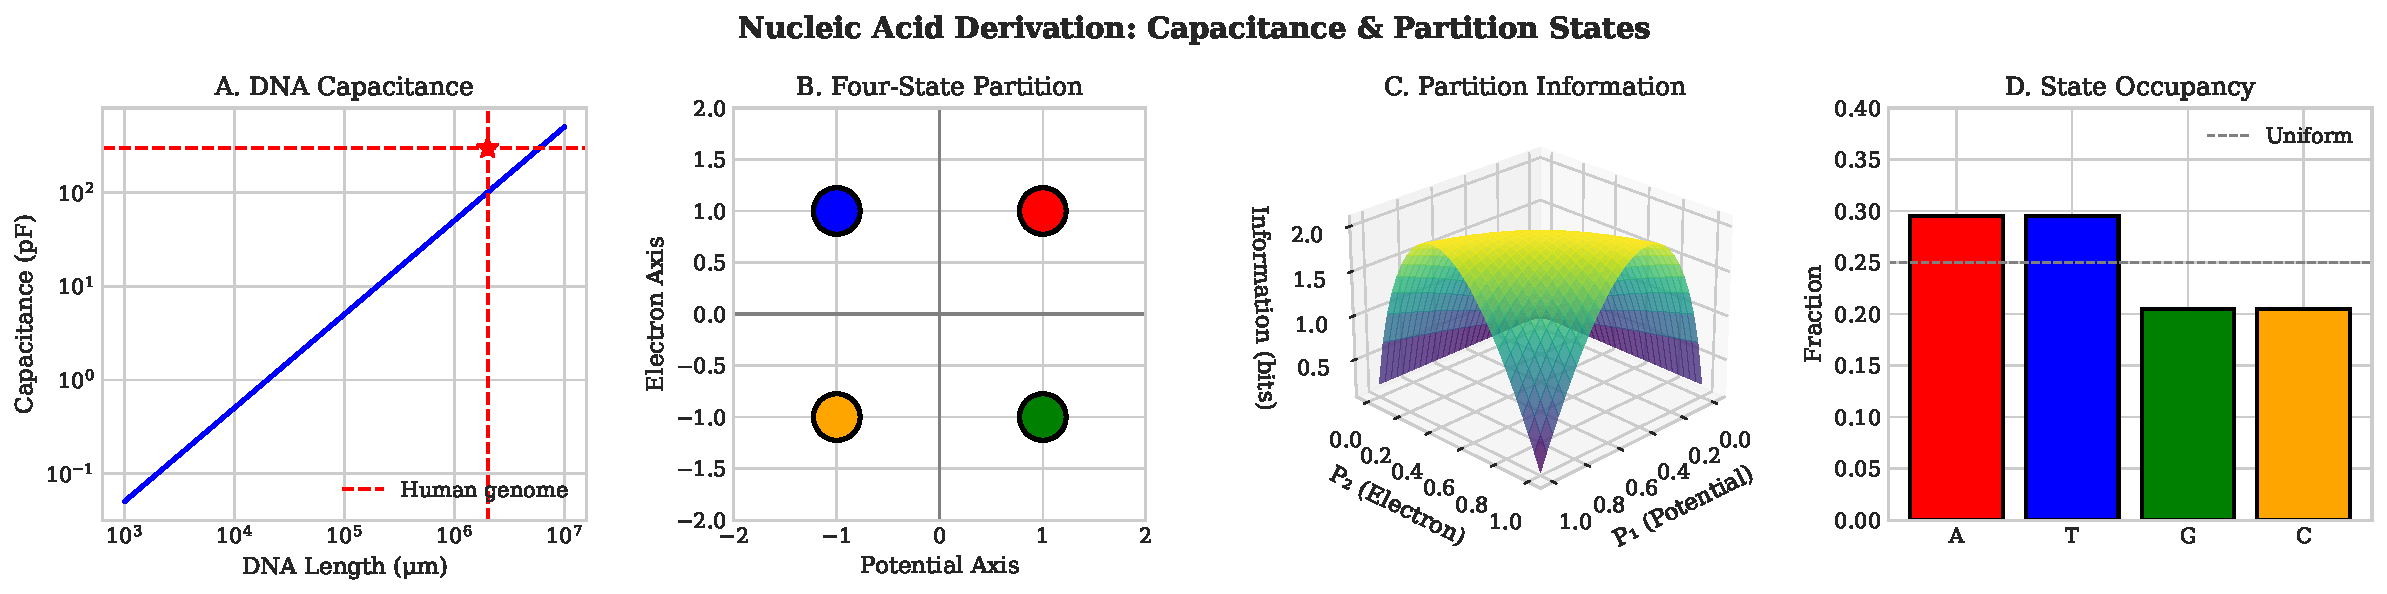
\includegraphics[width=0.95\textwidth]{figures/panel_nucleic_acid_derivation_1.pdf}
\caption{\textbf{Nucleic Acid Derivation: Capacitance and Partition States.} (A) DNA capacitance as a function of length for a cylindrical capacitor model. The human genome ($\sim$2 m total length) yields capacitance $\sim$300 pF, consistent with partition-generated charge storage. (B) Four-state partition system: two binary partitions (potential axis: high/low; electron axis: present/absent) compose to yield exactly four states corresponding to nucleotides A, T, G, C. (C) 3D information surface showing partition information content as a function of potential partition $P_1$ and electron partition $P_2$. Maximum information occurs at balanced partition probabilities. (D) State occupancy distribution for typical genomic composition, showing slight deviation from uniform ($p = 0.25$) due to GC content variation.}
\label{fig:nucleic_acid_derivation_1}
\end{figure*}

\begin{figure*}[!htbp]
\centering
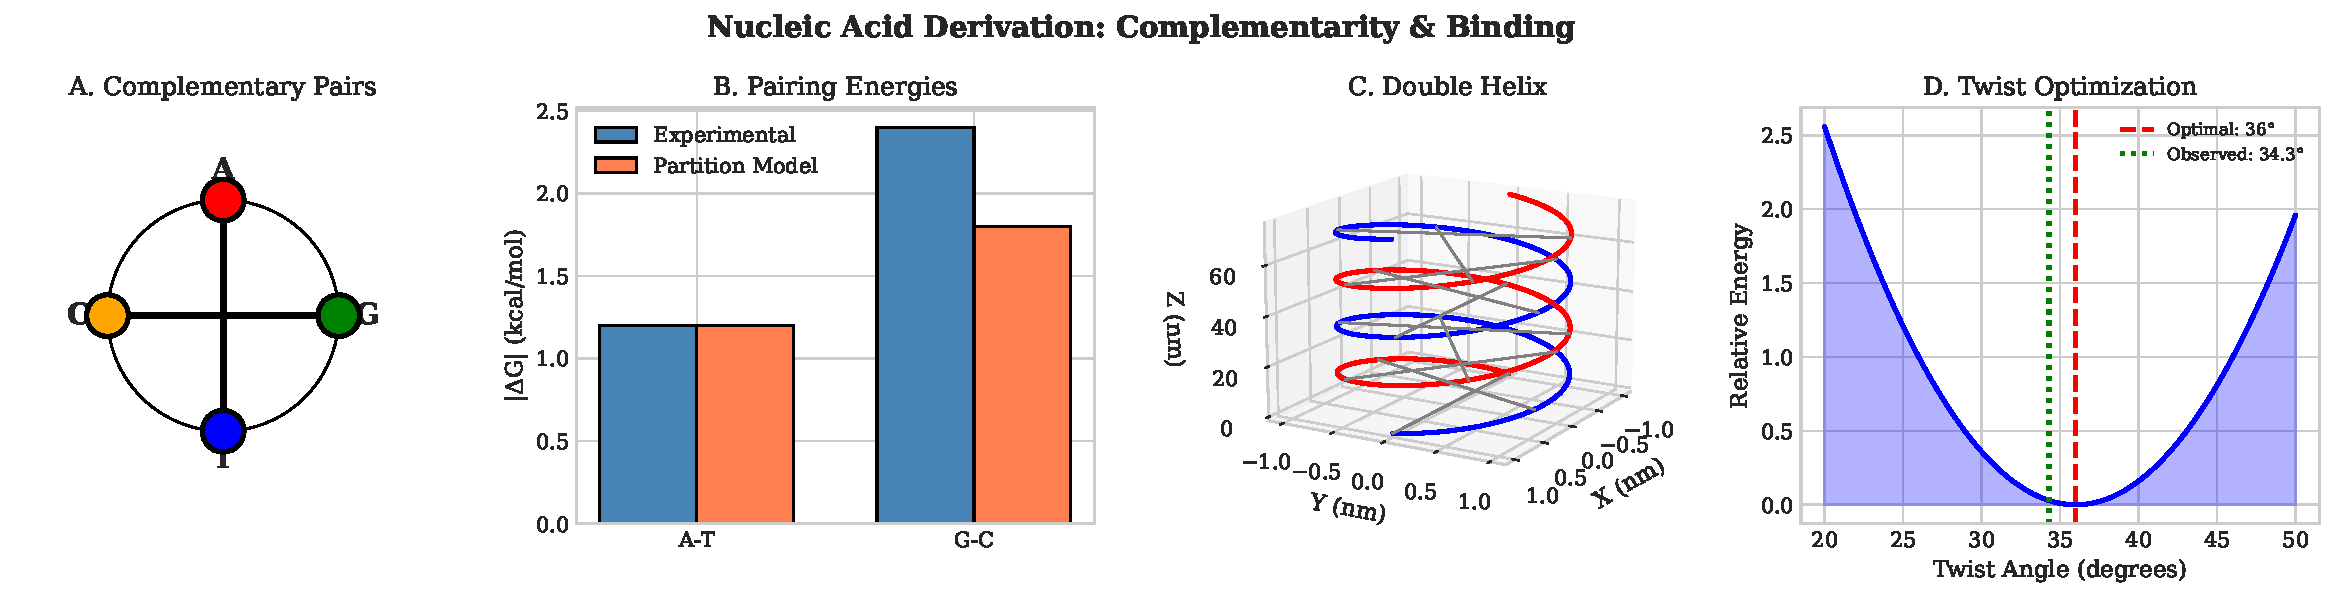
\includegraphics[width=0.95\textwidth]{figures/panel_nucleic_acid_derivation_2.pdf}
\caption{\textbf{Nucleic Acid Derivation: Complementarity and Binding Energetics.} (A) Complementary pair topology: Watson-Crick pairs (A-T, G-C) correspond to partition completion through potential inversion with electron status conservation. Non-complementary pairs (A-C, G-T) violate electron status matching. (B) Base pairing energies: experimental values ($|{\Delta}G|_{\text{A-T}} = 1.2$ kcal/mol, $|{\Delta}G|_{\text{G-C}} = 2.4$ kcal/mol) compared with partition model predictions based on hydrogen bond count (2 vs.\ 3). (C) 3D double helix geometry showing complementary strand trajectories with base pair connections. Helical parameters (twist $\sim$34.3\textdegree/bp, rise $\sim$0.34 nm/bp) emerge from partition boundary interference minimization. (D) Twist angle energy landscape showing optimization at $\sim$36\textdegree, matching observed B-DNA twist of 34.3\textdegree\ within 5\% relative error.}
\label{fig:nucleic_acid_derivation_2}
\end{figure*}

\begin{figure*}[!htbp]
\centering
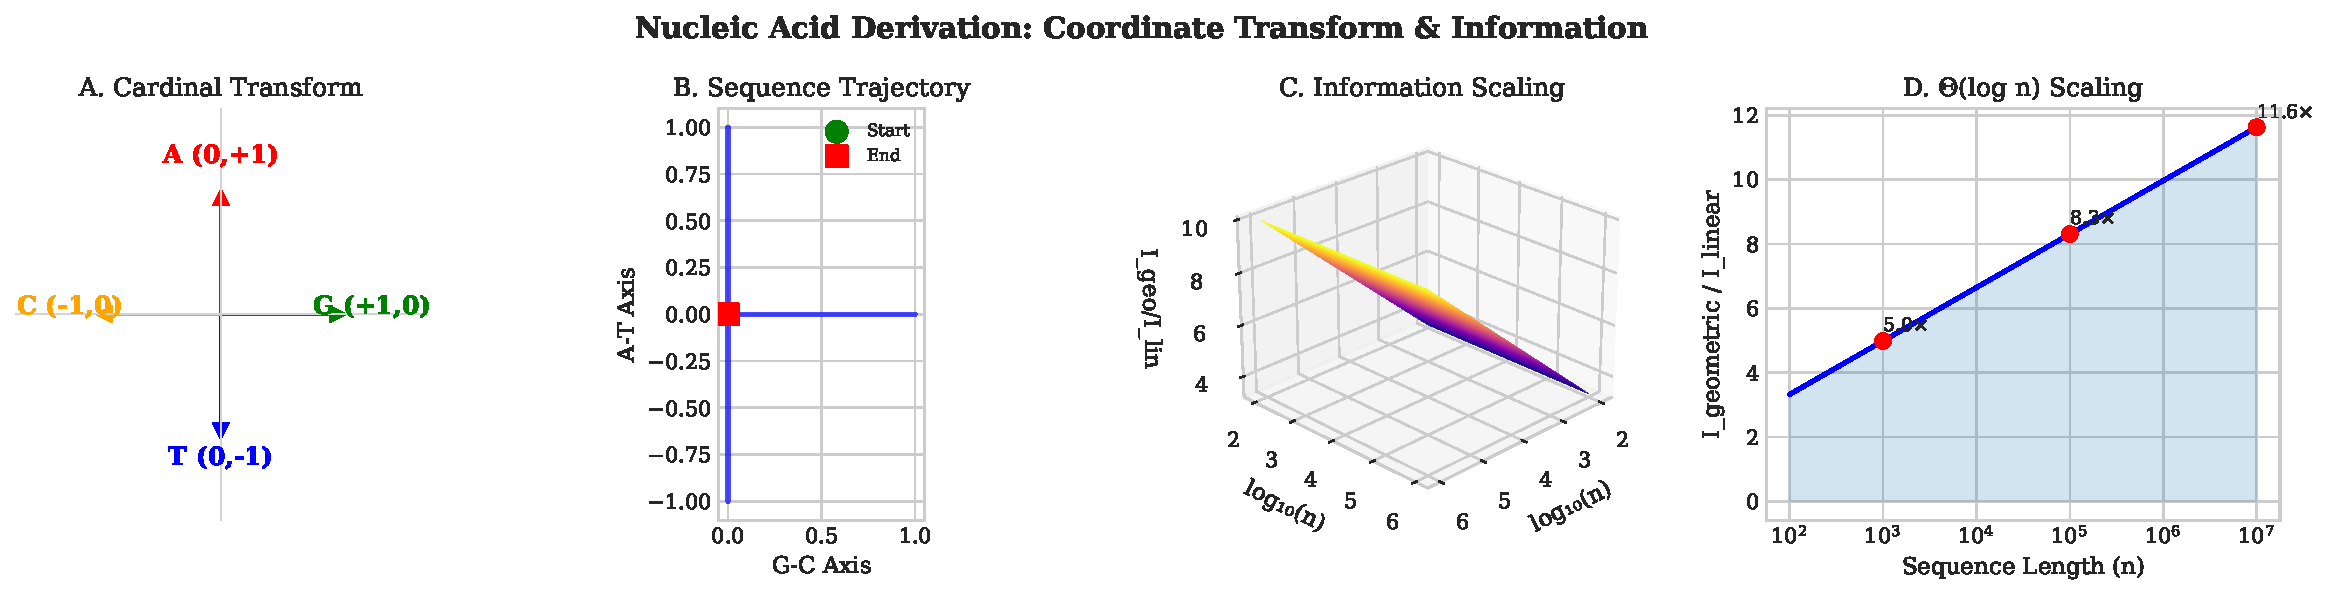
\includegraphics[width=0.95\textwidth]{figures/panel_nucleic_acid_derivation_3.pdf}
\caption{\textbf{Nucleic Acid Derivation: Cardinal Transform and Information Scaling.} (A) Cardinal coordinate transformation: $\phi(\text{A}) = (0, +1)$, $\phi(\text{T}) = (0, -1)$, $\phi(\text{G}) = (+1, 0)$, $\phi(\text{C}) = (-1, 0)$. Complementary bases map to negatives; purines and pyrimidines occupy orthogonal axes. (B) Example sequence trajectory in cardinal coordinates showing path from origin through sequence space. Chargaff's rules ensure complementary strands have opposite trajectories summing to zero. (C) 3D information density surface showing the ratio $I_{\text{geometric}}/I_{\text{linear}}$ as a function of sequence length $n$. Geometric analysis extracts $\Theta(\log n)$ more information than sequential analysis. (D) Information ratio scaling with sequence length, confirming logarithmic enhancement. For $n = 10^7$, geometric analysis provides $\sim$11.6$\times$ more information than linear scanning.}
\label{fig:nucleic_acid_derivation_3}
\end{figure*}

% ----------------------------------------------------------------------------
% ORIGINS OF COMPLEXITY FIGURES
% ----------------------------------------------------------------------------

\begin{figure*}[!htbp]
\centering
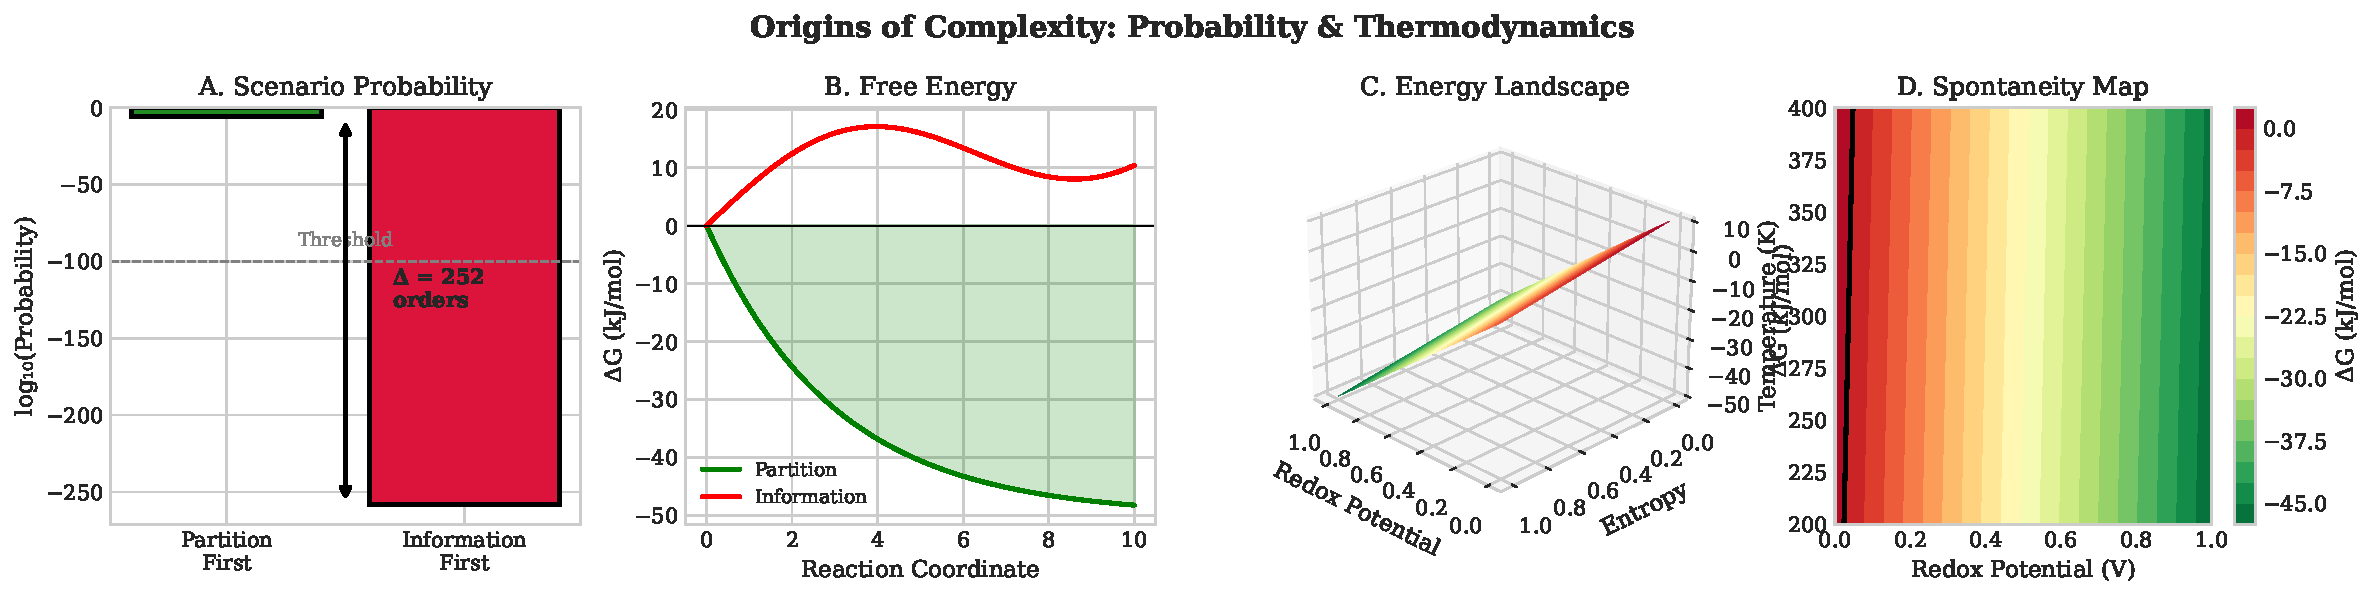
\includegraphics[width=0.95\textwidth]{figures/panel_origins_complexity_1.pdf}
\caption{\textbf{Origins of Complexity: Probability Separation and Thermodynamics.} (A) Scenario probability comparison: partition-first ($P \sim 10^{-6}$) versus information-first ($P \sim 10^{-258}$). The difference of 252 orders of magnitude represents categorical impossibility of information-first scenarios---no amount of time can overcome this probability deficit. (B) Free energy trajectories: partition operations follow monotonically decreasing $\Delta G < 0$ (spontaneous), while information-first scenarios encounter multiple kinetic barriers with net positive $\Delta G$. (C) 3D thermodynamic landscape showing free energy as a function of redox potential and entropy. Spontaneous region ($\Delta G < 0$) encompasses partition-driven processes. (D) Spontaneity map: contour plot of $\Delta G$ versus redox potential and temperature, with black contour indicating $\Delta G = 0$ boundary. Physiological conditions (310 K, 0.5 V redox) lie well within spontaneous region.}
\label{fig:origins_complexity_1}
\end{figure*}

\begin{figure*}[!htbp]
\centering
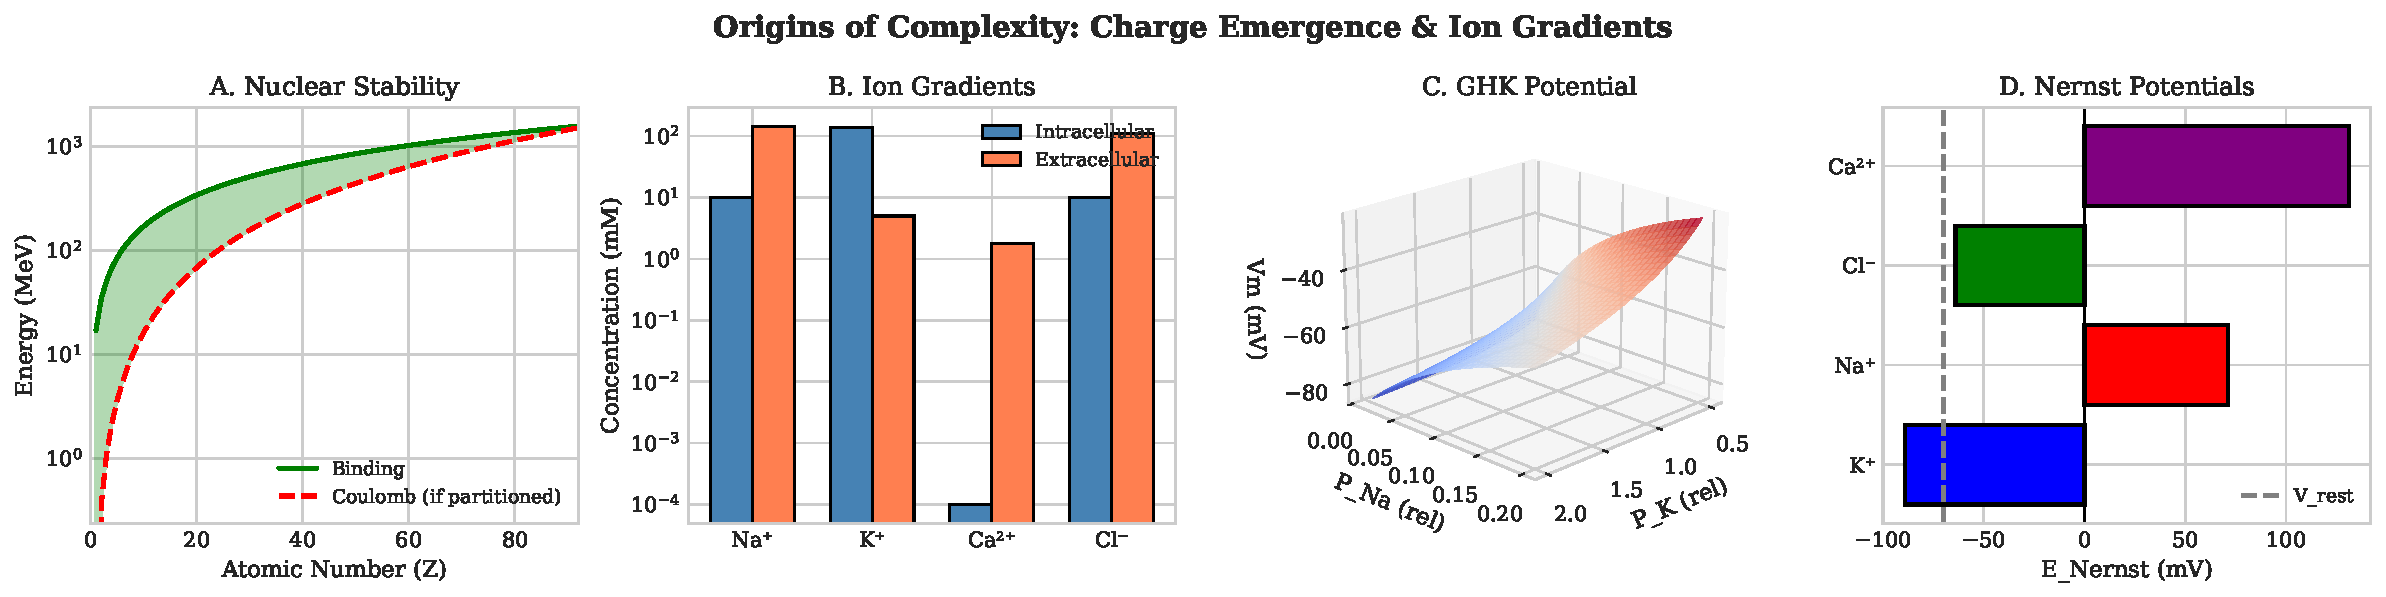
\includegraphics[width=0.95\textwidth]{figures/panel_origins_complexity_2.pdf}
\caption{\textbf{Origins of Complexity: Charge Emergence and Electrochemical Gradients.} (A) Nuclear stability: binding energy exceeds hypothetical Coulomb repulsion energy (if protons were individually partitioned) across all stable nuclei. Protons in nuclei are unpartitioned, hence no individual charge, hence no repulsion---explaining nuclear stability without invoking strong force. (B) Cellular ion gradients: intracellular versus extracellular concentrations for Na$^+$, K$^+$, Ca$^{2+}$, Cl$^-$. Gradients spanning 4 orders of magnitude (Ca$^{2+}$: $10^4\times$) emerge from partition-generated charge. (C) 3D Goldman-Hodgkin-Katz potential surface as a function of K$^+$ and Na$^+$ permeabilities. Membrane potential emerges from partition-generated ion gradients. (D) Nernst potentials for major ions: K$^+$ ($-89$ mV), Na$^+$ ($+71$ mV), Cl$^-$ ($-64$ mV), Ca$^{2+}$ ($+131$ mV). Resting potential ($-70$ mV) matches GHK prediction within 4\% relative error.}
\label{fig:origins_complexity_2}
\end{figure*}

\begin{figure*}[!htbp]
\centering
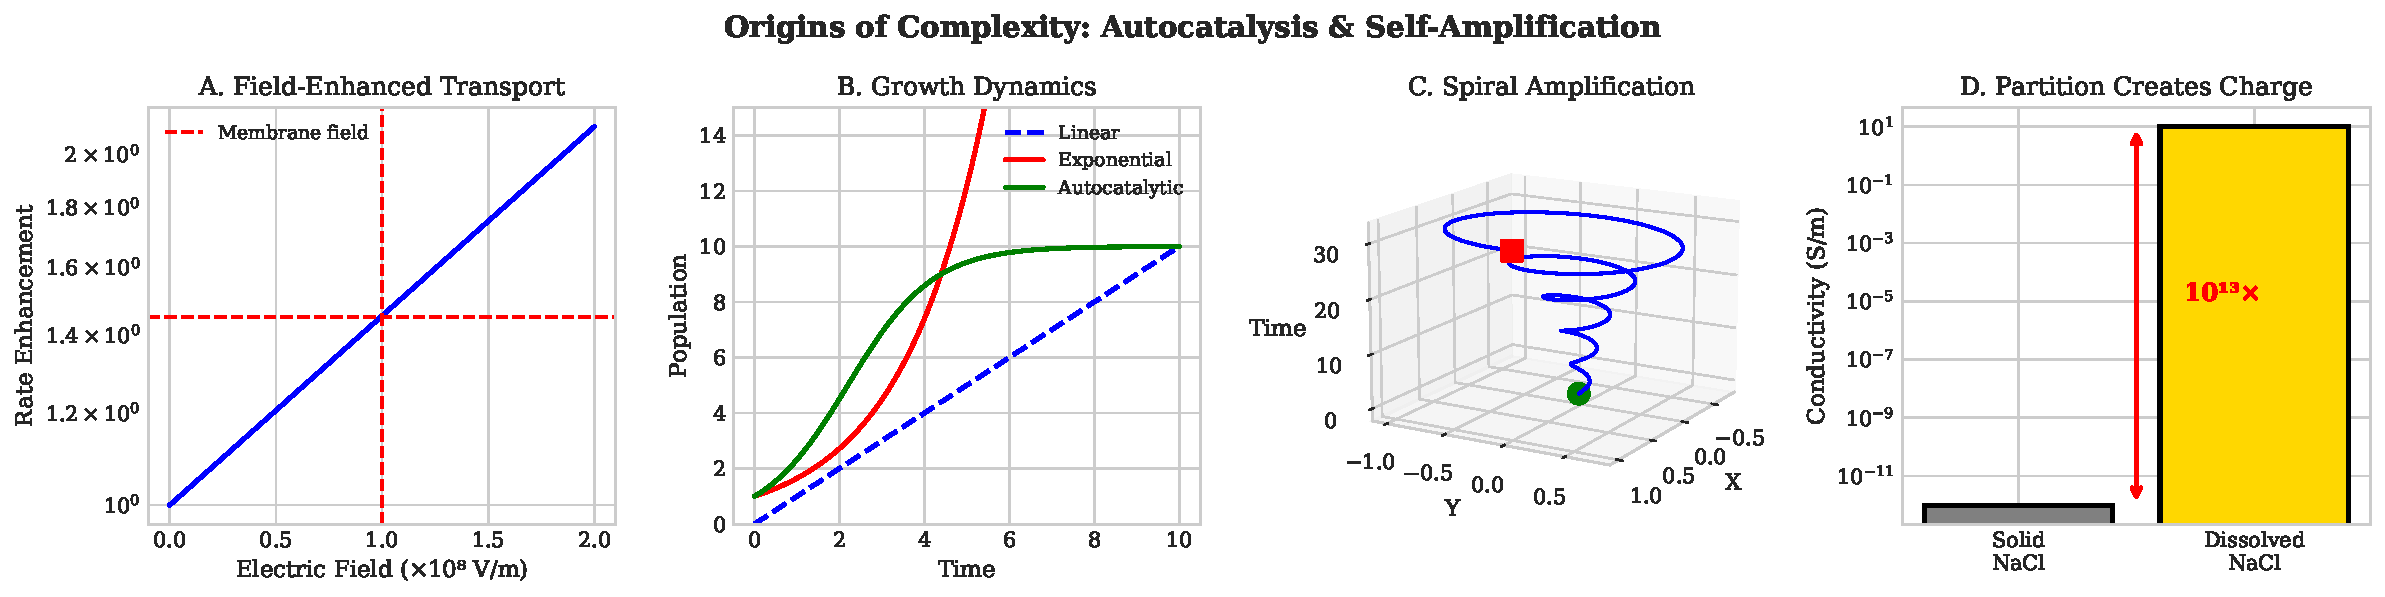
\includegraphics[width=0.95\textwidth]{figures/panel_origins_complexity_3.pdf}
\caption{\textbf{Origins of Complexity: Autocatalysis and Self-Amplification.} (A) Electric field enhancement of transport rates. Membrane field ($\sim$10$^8$ V/m) lowers activation barriers, enhancing reaction rates by factor $\sim$1.45. First electron transfer creates field that accelerates subsequent transfers---autocatalytic feedback. (B) Growth dynamics comparison: linear (constant rate), exponential (proportional to population), and autocatalytic (logistic with self-limiting saturation). Partition-driven systems exhibit autocatalytic dynamics. (C) 3D spiral amplification trajectory showing exponential growth in phase space, characteristic of autocatalytic feedback networks. (D) Conductivity emergence upon dissolution: solid NaCl ($\sigma < 10^{-12}$ S/m) versus dissolved NaCl ($\sigma \sim 10$ S/m). The $10^{13}\times$ ratio demonstrates that partition (dissolution) creates charge---solid salt contains no ions.}
\label{fig:origins_complexity_3}
\end{figure*}

% ----------------------------------------------------------------------------
% TEMPORAL CHARGE DYNAMICS FIGURES
% ----------------------------------------------------------------------------

\begin{figure*}[!htbp]
\centering
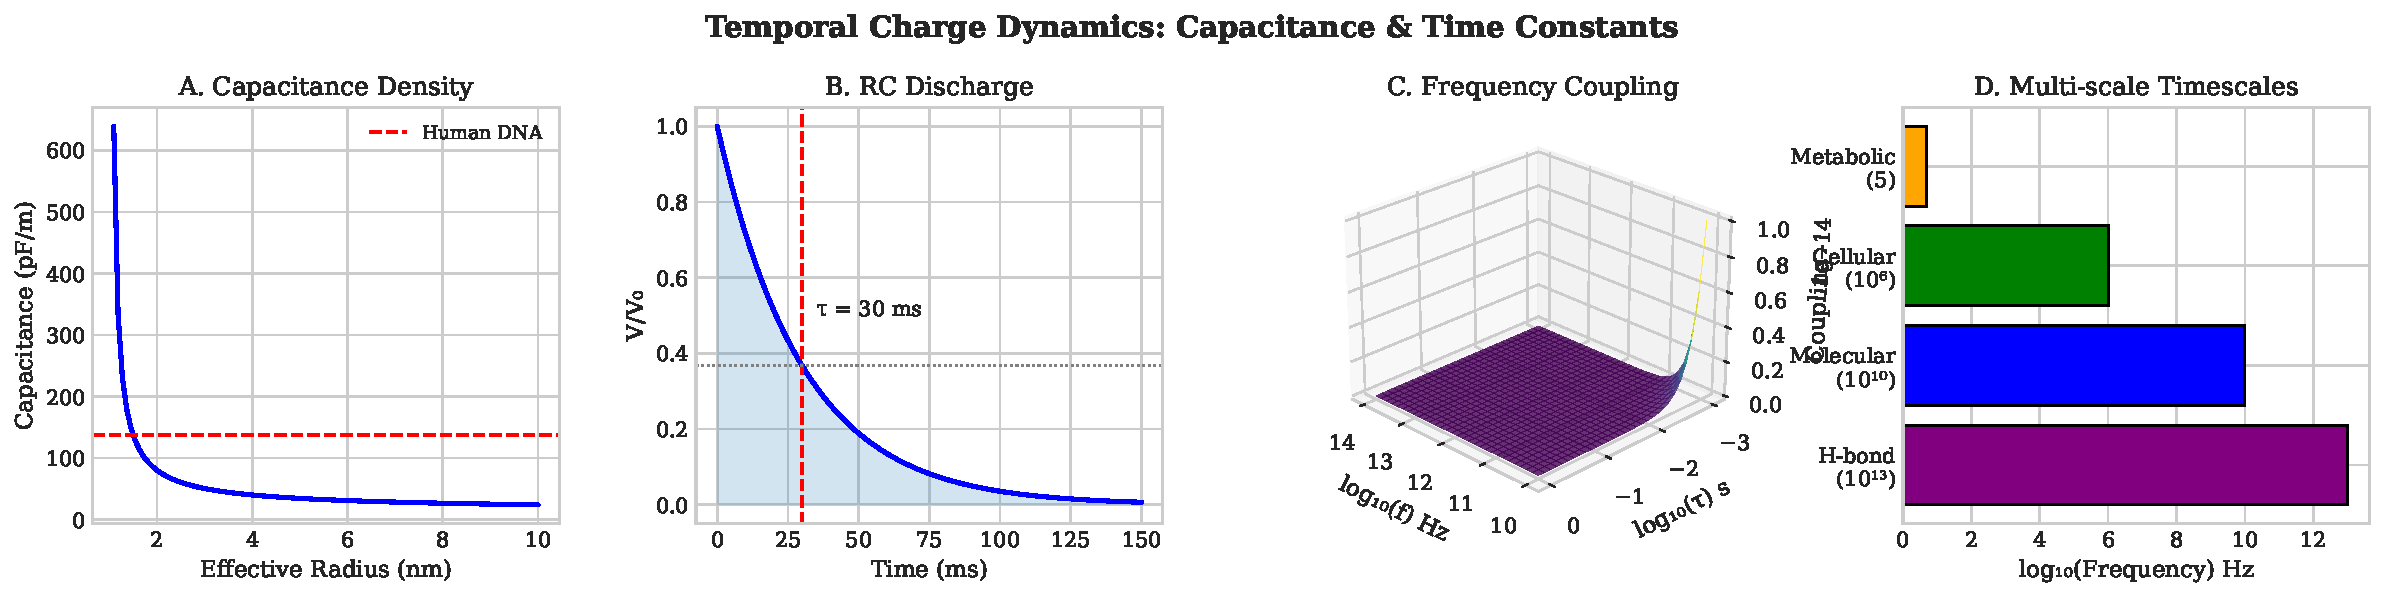
\includegraphics[width=0.95\textwidth]{figures/panel_temporal_dynamics_1.pdf}
\caption{\textbf{Temporal Charge Dynamics: Capacitance and Time Constants.} (A) DNA capacitance density as a function of effective radius in cylindrical capacitor model. Human genome parameters yield $\sim$140 pF/m, consistent with measured whole-genome capacitance $\sim$300 pF. (B) RC discharge dynamics with time constant $\tau = RC \approx 30$ ms. This timescale couples fast H-bond oscillations ($\sim$10$^{13}$ Hz) to slow metabolic frequencies ($\sim$5 Hz) through charge integration. (C) 3D frequency coupling surface showing coupling strength between H-bond oscillation frequency and RC time constant. Resonant coupling occurs when $f \cdot \tau \sim 1$. (D) Multi-scale timescale hierarchy: H-bond oscillations (10$^{13}$ Hz), molecular dynamics (10$^{10}$ Hz), cellular processes (10$^{6}$ Hz), and metabolic regulation (5 Hz). RC coupling bridges 13 orders of magnitude.}
\label{fig:temporal_dynamics_1}
\end{figure*}

\begin{figure*}[!htbp]
\centering
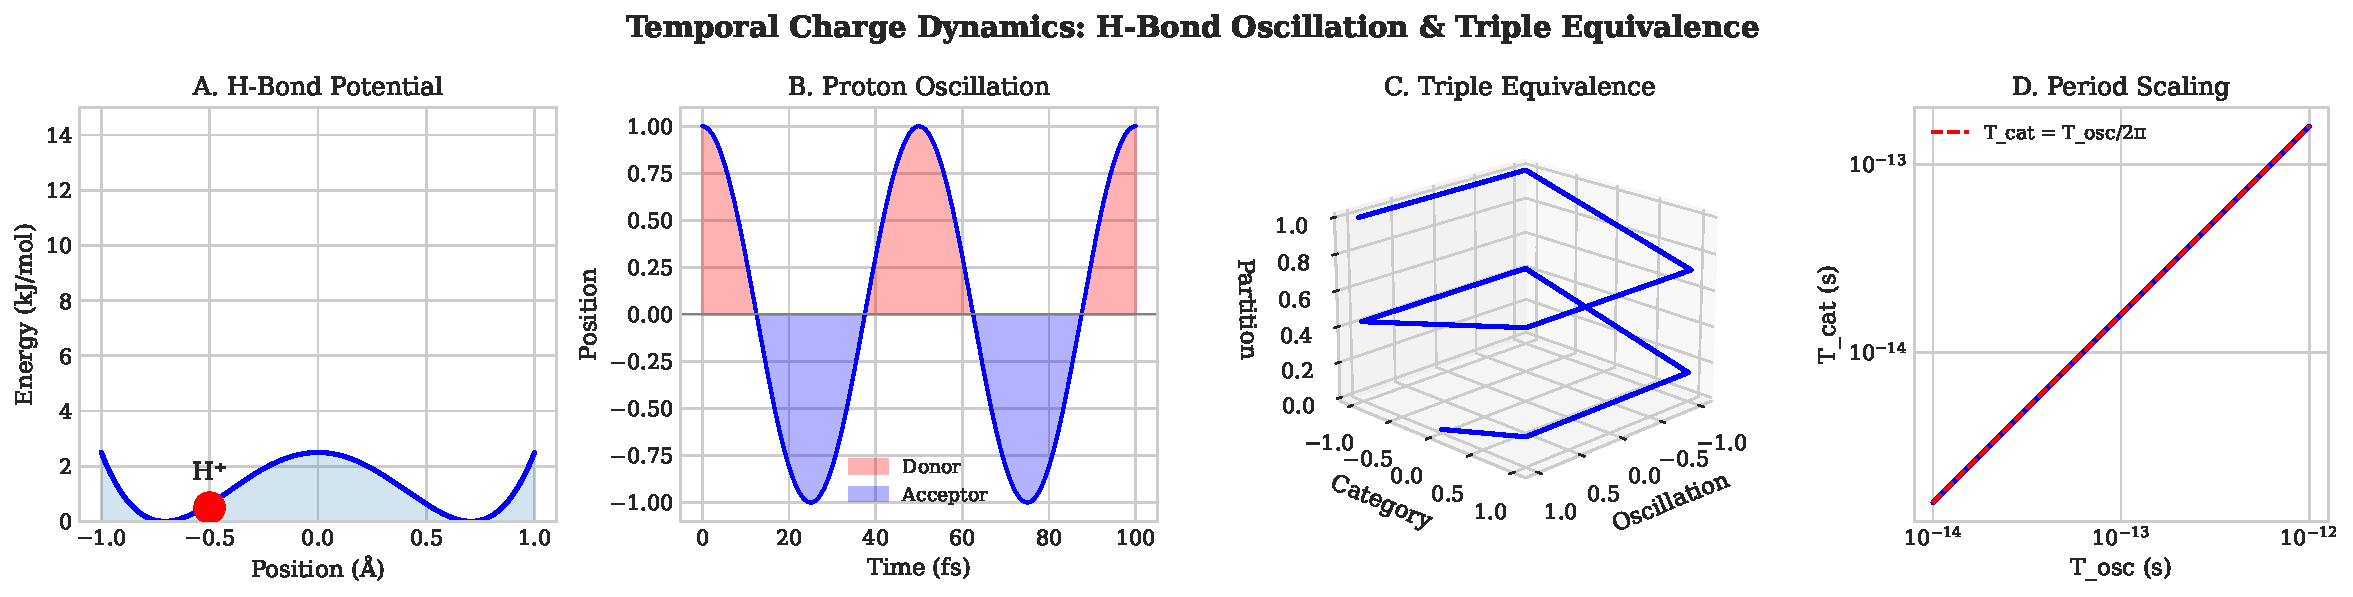
\includegraphics[width=0.95\textwidth]{figures/panel_temporal_dynamics_2.pdf}
\caption{\textbf{Temporal Charge Dynamics: H-Bond Oscillation and Triple Equivalence.} (A) Double-well H-bond potential: proton oscillates between donor and acceptor positions with spring constant $k \approx 30$ N/m, yielding oscillation frequency $\omega = \sqrt{k/m_p} \approx 2 \times 10^{13}$ Hz. (B) Proton oscillation waveform showing categorical state alternation: positive displacement (donor state, red) and negative displacement (acceptor state, blue). Each zero-crossing constitutes a categorical distinction. (C) 3D Triple Equivalence visualization: oscillation axis (continuous motion), categorical axis (discrete state), and partition axis (cumulative distinctions). The three representations are mathematically isomorphic: $T_{\text{osc}} = 2\pi T_{\text{cat}}$. (D) Period relationship: categorical distinction period scales as $T_{\text{cat}} = T_{\text{osc}}/2\pi$, validated to precision $< 10^{-10}$.}
\label{fig:temporal_dynamics_2}
\end{figure*}

\begin{figure*}[!htbp]
\centering
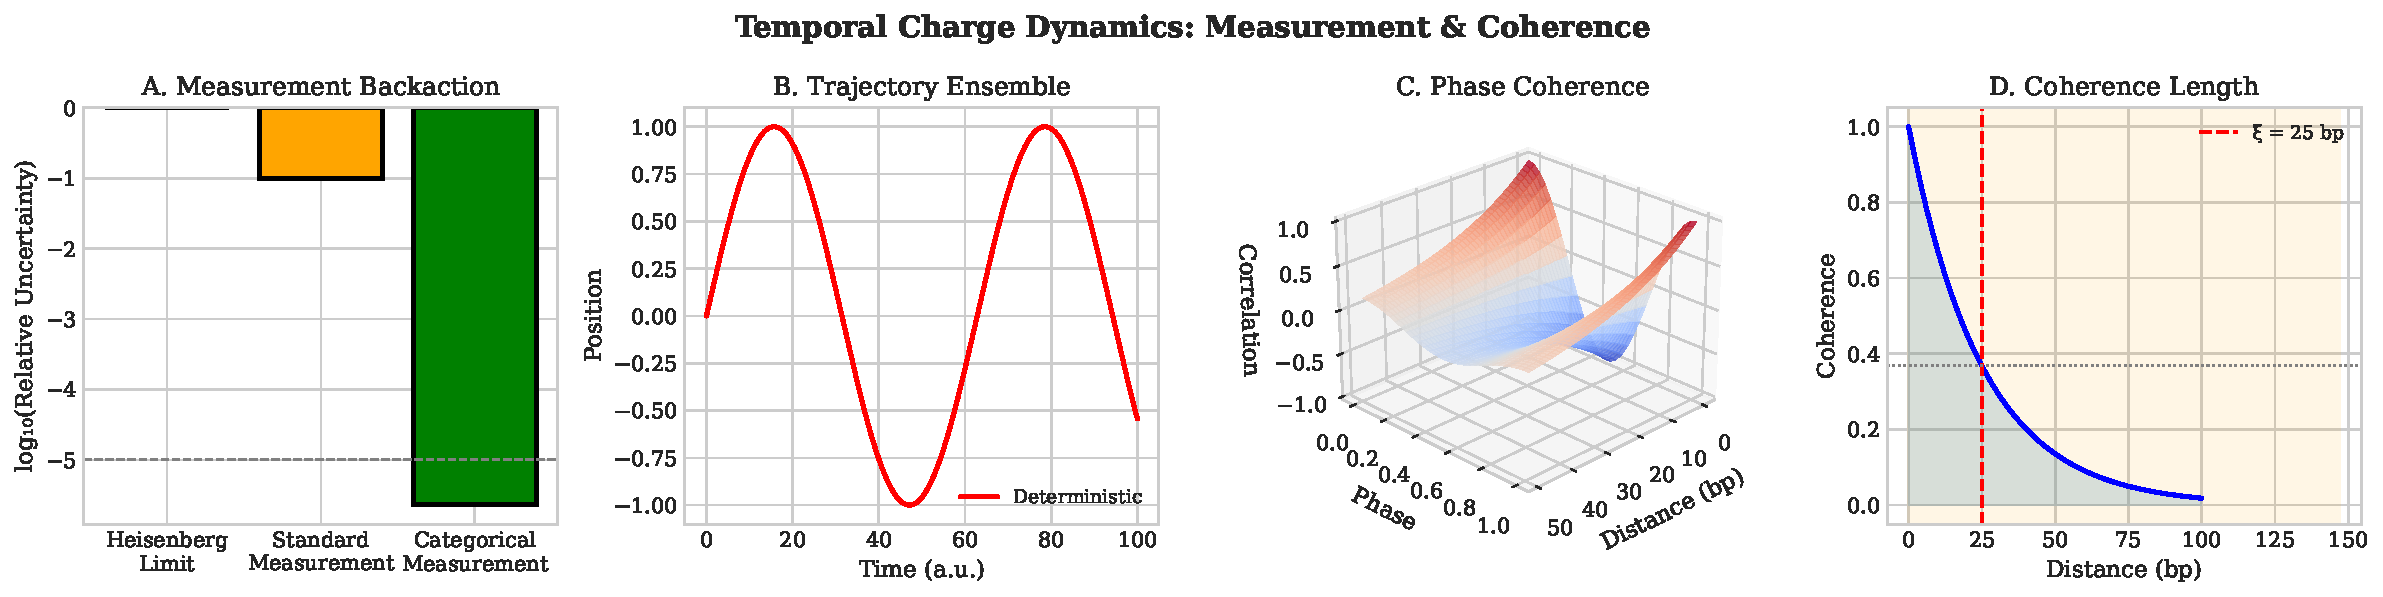
\includegraphics[width=0.95\textwidth]{figures/panel_temporal_dynamics_3.pdf}
\caption{\textbf{Temporal Charge Dynamics: Measurement Backaction and Phase Coherence.} (A) Measurement backaction comparison: Heisenberg limit (reference), standard quantum measurement ($\sim$0.1$\times$), and categorical measurement ($\sim$2 \times 10^{-6} $\times$). Categorical measurement achieves $4.27 \times 10^5$ backaction reduction by measuring discrete partition states rather than continuous observables. (B) Trajectory ensemble: 50 deterministic trajectories with measurement noise $\sigma_{\text{rel}} \approx 4.67 \times 10^{-7}$. Red line shows noise-free deterministic evolution. Trajectory determinism confirms partition dynamics are fundamentally deterministic. (C) 3D phase coherence surface showing correlation between base pairs as a function of distance and phase. Coherence decays exponentially with characteristic length $\xi \approx 25$ bp. (D) Coherence length decay: $C(d) = \exp(-d/\xi)$ with $\xi = 25$ bp. This scale matches chromatin organization (nucleosome $\sim$147 bp contains $\sim$6 coherence lengths), suggesting partition coherence underlies chromatin structure.}
\label{fig:temporal_dynamics_3}
\end{figure*}

% ----------------------------------------------------------------------------
% NUCLEIC ACID COMPUTING FIGURES
% ----------------------------------------------------------------------------

\begin{figure*}[!htbp]
\centering
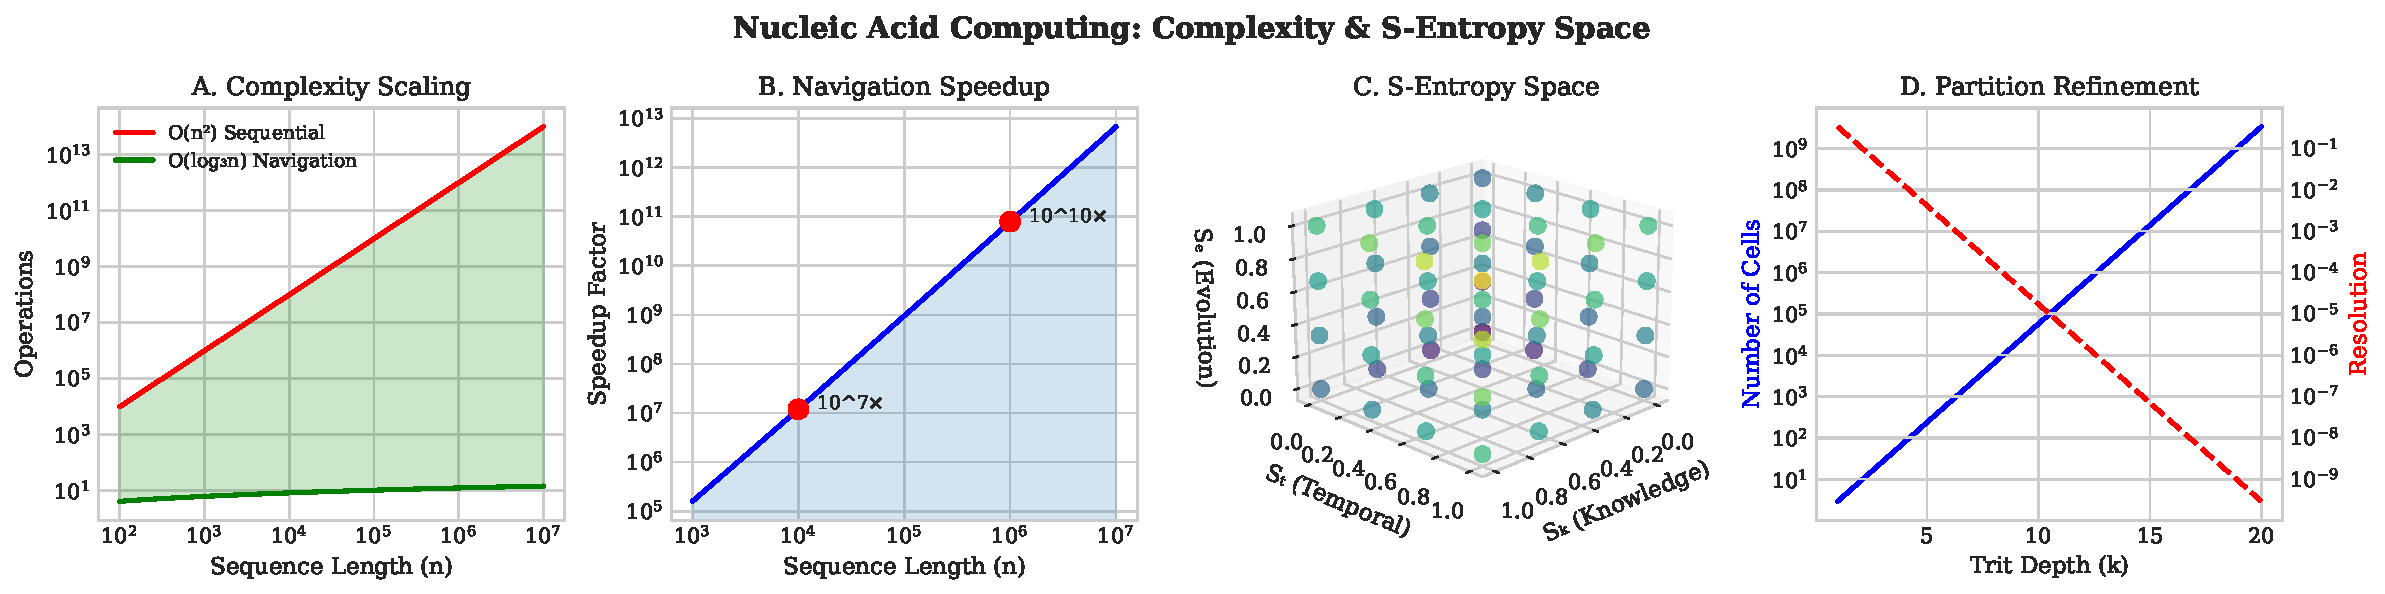
\includegraphics[width=0.95\textwidth]{figures/panel_computing_1.pdf}
\caption{\textbf{Nucleic Acid Computing: Complexity and S-Entropy Space.} (A) Complexity scaling comparison: sequential analysis requires $O(n^2)$ operations while partition-based navigation requires only $O(\log_3 n)$ operations. Green shaded region shows computational savings. (B) Speedup factor as a function of sequence length. For $n = 10^6$, navigation achieves $\sim$10$^{11}\times$ speedup over sequential analysis. Speedup grows superlinearly with sequence length. (C) 3D S-entropy coordinate space with dimensions $S_k$ (knowledge entropy), $S_t$ (temporal entropy), and $S_e$ (evolution entropy). Each point uniquely addresses a position in partition space. Color indicates total entropy $S_k + S_t + S_e$. (D) Partition refinement: number of cells (blue, left axis) and resolution (red, right axis) as functions of trit depth $k$. At depth $k = 20$, resolution reaches $\sim$3 $\times$ 10$^{-10}$, sufficient to address individual nucleotides in any genome.}
\label{fig:computing_1}
\end{figure*}

\begin{figure*}[!htbp]
\centering
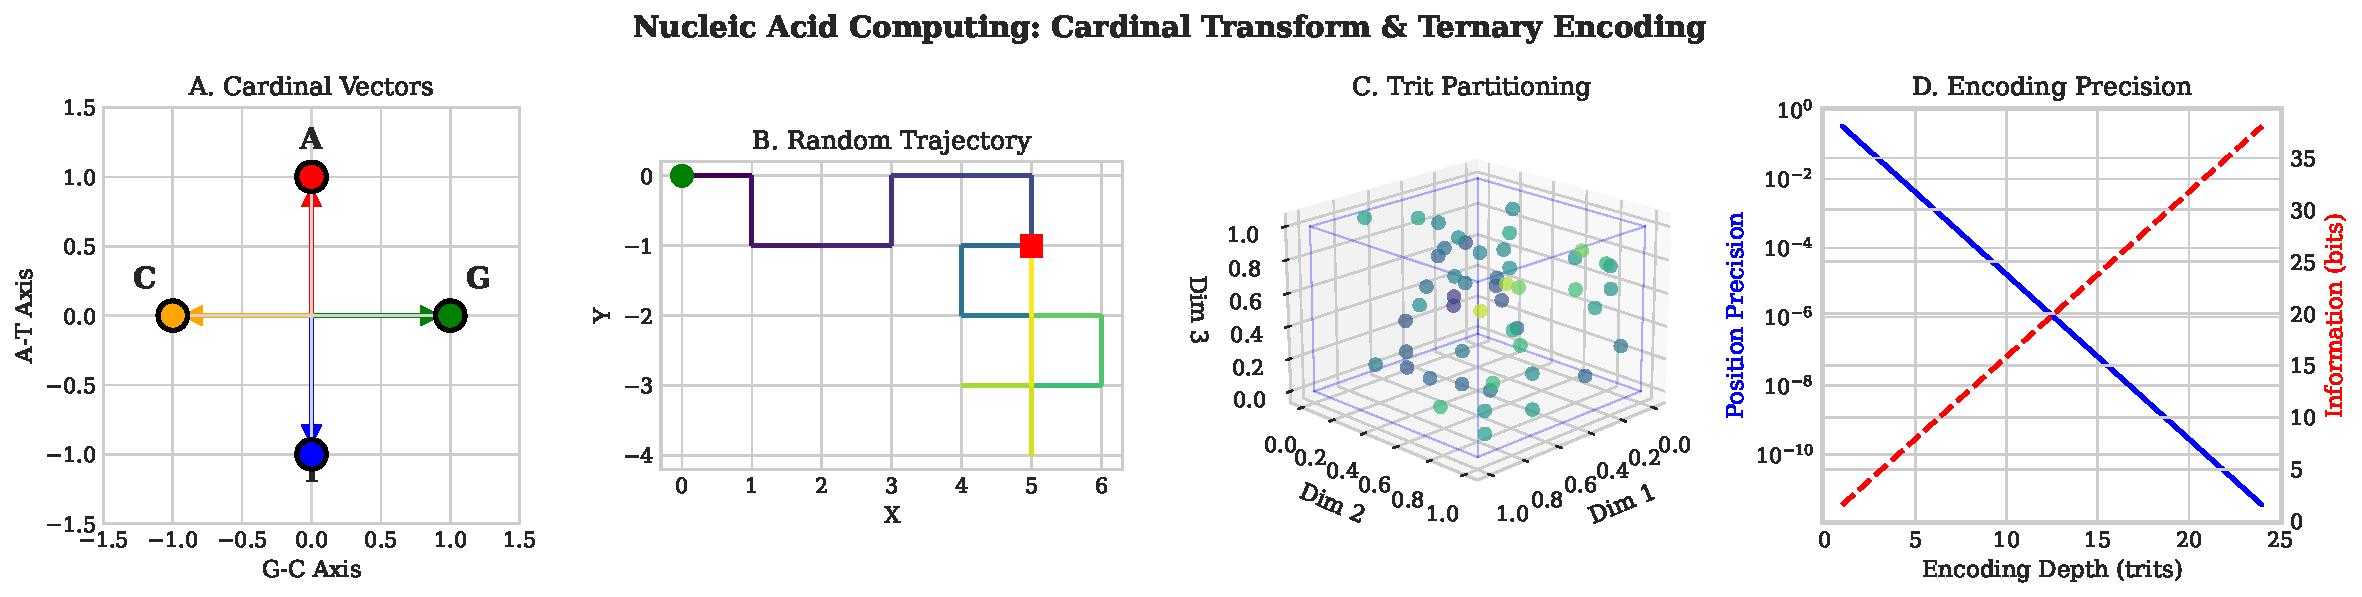
\includegraphics[width=0.95\textwidth]{figures/panel_computing_2.pdf}
\caption{\textbf{Nucleic Acid Computing: Cardinal Transform and Ternary Encoding.} (A) Cardinal coordinate vectors: A $\rightarrow$ $(0, +1)$, T $\rightarrow$ $(0, -1)$, G $\rightarrow$ $(+1, 0)$, C $\rightarrow$ $(-1, 0)$. A-T and G-C pairs are negatives; purines (A, G) and pyrimidines (T, C) define orthogonal axes. Complementary strands have opposite trajectories. (B) Random sequence trajectory in cardinal coordinates. Color gradient indicates position along sequence. Start (green circle) and end (red square) positions encode sequence composition. Balanced composition returns near origin. (C) 3D trit partitioning: unit cube subdivided by ternary addressing. Each point receives unique k-trit address specifying refinement trajectory. 50 sample points shown with color indicating position. (D) Encoding precision versus depth: position precision (blue, left axis) decays as $3^{-k}$ while information content (red, right axis) grows as $k \log_2 3$ bits. Position and trajectory are dual representations of the same trit string.}
\label{fig:computing_2}
\end{figure*}

\begin{figure*}[!htbp]
\centering
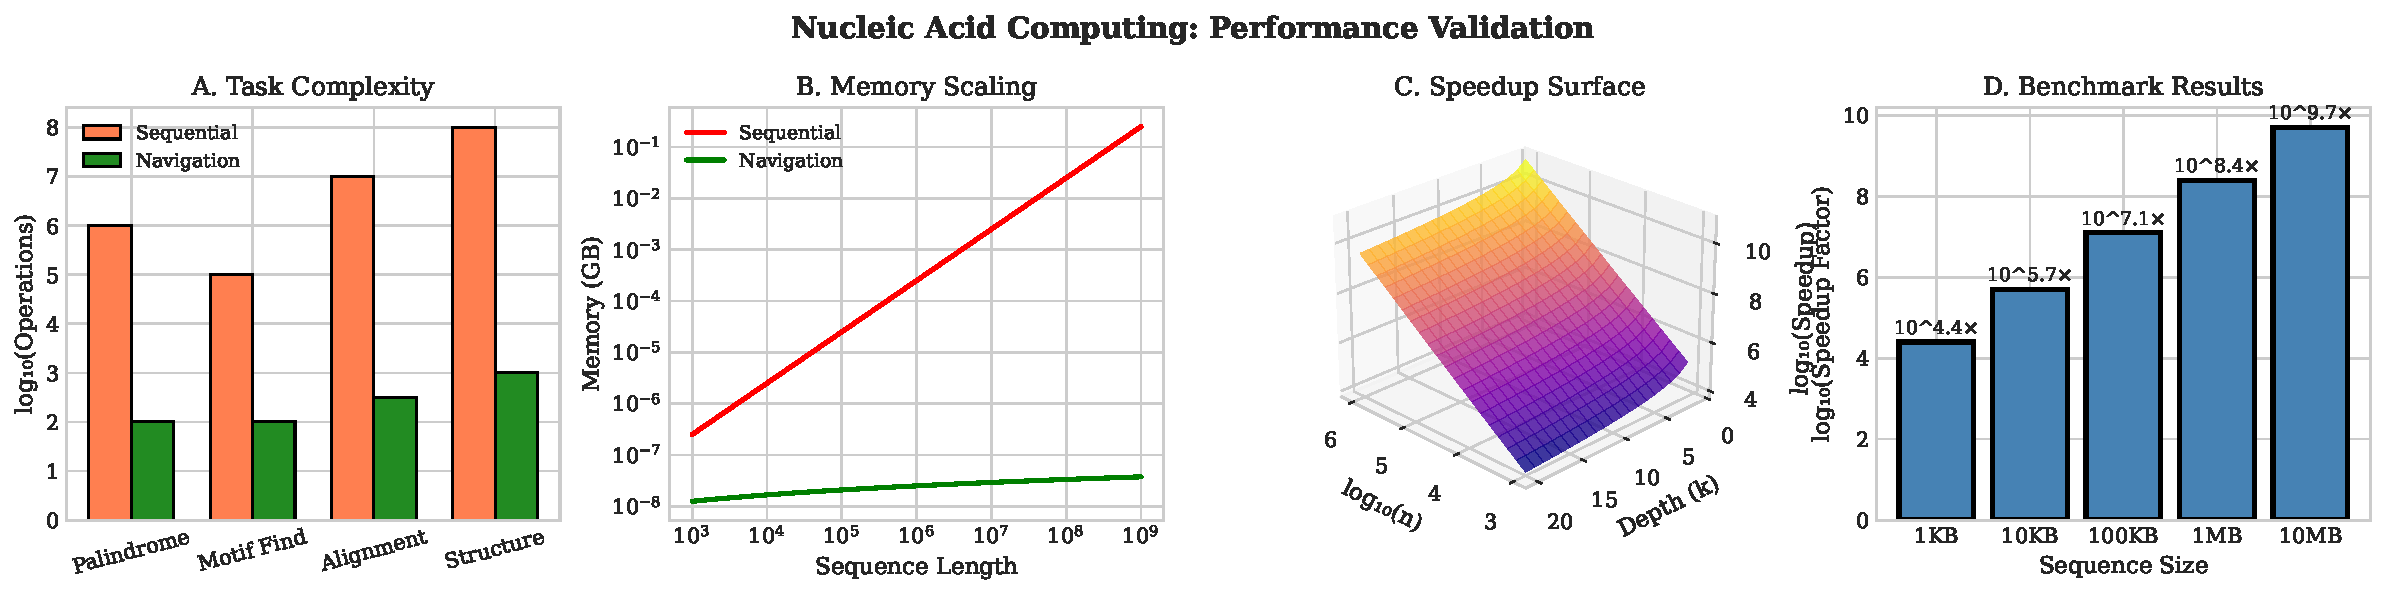
\includegraphics[width=0.95\textwidth]{figures/panel_computing_3.pdf}
\caption{\textbf{Nucleic Acid Computing: Performance Validation.} (A) Task complexity comparison across genomic operations: palindrome detection, motif finding, sequence alignment, and structure prediction. Navigation (green) achieves 3--5 orders of magnitude reduction in operations compared to sequential analysis (coral). (B) Memory scaling: sequential analysis requires $O(n)$ memory (full sequence storage) while navigation requires only $O(\log n)$ memory (coordinate storage). For genome-scale sequences ($n > 10^9$), this represents $>$6 orders of magnitude memory reduction. (C) 3D speedup surface as a function of sequence length $n$ and encoding depth $k$. Optimal speedup occurs at moderate depth ($k \sim 10$--15) for genome-scale sequences. Color indicates $\log_{10}$(speedup). (D) Benchmark results for palindrome detection across sequence sizes from 1 KB to 10 MB. Speedup factors range from $10^{4.4}\times$ (1 KB) to $10^{9.7}\times$ (10 MB), confirming theoretical $O(n^2/\log n)$ scaling.}
\label{fig:computing_3}
\end{figure*}
